\chapter{VHDL硬件综合专题}

\section{学习目标}

不是学VHDL语法。而是理解：

\begin{center}
\fbox{%
\begin{minipage}{0.85\textwidth}
\textbf{你写的每一行VHDL，最终在FPGA中变成了什么硬件？}
\end{minipage}%
}
\end{center}

\section{if-else 综合成什么}

\begin{lstlisting}[caption={if-else示例}]
 if sel = '1' then
  y <= a;
else
  y <= b;
end if;
\end{lstlisting}

\textbf{综合结果：MUX（数据选择器）}

\begin{center}
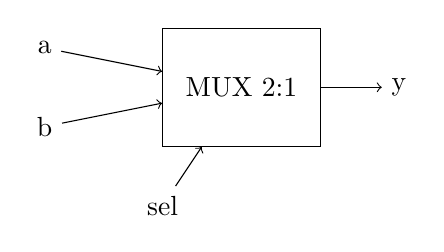
\begin{tikzpicture}
  \node[draw, minimum width=2cm, minimum height=1.5cm] (mux) at (0,0) {MUX 2:1};
  \node (a) at (-2.5,0.5) {a};
  \node (b) at (-2.5,-0.5) {b};
  \node (sel) at (-1,-1.5) {sel};
  \node (y) at (2,0) {y};
  \draw[->] (a) -- (mux);
  \draw[->] (b) -- (mux);
  \draw[->] (sel) -- (mux);
  \draw[->] (mux) -- (y);
\end{tikzpicture}
\end{center}

\subsection{if-else级联}

\begin{lstlisting}
 if sel = "00" then
  y <= d0;
elsif sel = "01" then
  y <= d1;
elsif sel = "10" then
  y <= d2;
else
  y <= d3;
end if;
\end{lstlisting}

\textbf{综合结果：优先级编码的选择器（级联MUX）}。sel=11优先级最低（在最后的else中），综合工具可能优化为并行MUX。

\begin{keypoint}[if-else与硬件]
\textbf{if-else} → \textbf{优先级逻辑}（如优先级编码器、级联MUX）

条件从上到下优先级递减。

如果条件互斥，综合工具常优化为并行case结构。
\end{keypoint}

\section{case 综合成什么}

\begin{lstlisting}
case sel is
  when "00" => y <= d0;
  when "01" => y <= d1;
  when "10" => y <= d2;
  when "11" => y <= d3;
end case;
\end{lstlisting}

\textbf{综合结果：并行MUX（所有分支并行判断）}

与if-else不同，case的所有分支\textbf{并行}判断，没有优先级。

\begin{keypoint}[case与硬件]
\textbf{case} → \textbf{并行选择器} / \textbf{译码器结构}

所有分支地位平等，综合器生成并行比较逻辑。

适用于：
\begin{itemize}
  \item MUX（选择器）
  \item 译码器
  \item 状态机的状态转移
  \item 查找表
\end{itemize}
\end{keypoint}

\section{process 综合成什么}

\begin{lstlisting}
process(clk)
begin
  if rising_edge(clk) then
    q <= d;
  end if;
end process;
\end{lstlisting}

\textbf{process块本身不产生硬件。} process只是一种描述方式。

\textbf{process内部的逻辑} 决定综合成什么：
\begin{itemize}
  \item 有clk边沿检测 → 产生D触发器/寄存器
  \item 纯组合逻辑（无clk）→ 产生组合逻辑门
  \item 带异步复位 → D触发器 + 复位逻辑
\end{itemize}

\begin{keypoint}[process与硬件]
\textbf{process} = 硬件描述的容器（本身不是硬件）

\textbf{process(CLK)} + \texttt{rising\_edge} → \textbf{D触发器/寄存器组}

\textbf{process(全部输入)} + 无clk → \textbf{组合逻辑}

\textbf{决定硬件的是process内部的代码}，不是process本身。
\end{keypoint}

\section{signal 对应什么硬件}

\begin{lstlisting}
signal x : std_logic;
signal data : std_logic_vector(7 downto 0);
\end{lstlisting}

\textbf{signal = 一根线（组合逻辑）或一个寄存器（时序逻辑）}

\begin{itemize}
  \item \texttt{signal x : std\_logic} → 1根物理连线 或 1个D触发器
  \item \texttt{signal data : std\_logic\_vector(7 downto 0)} → 8根线 或 8个D触发器
\end{itemize}

\textbf{关键判断}：signal是线还是寄存器？

\begin{center}
\begin{tabular}{|l|l|}
\hline
\textbf{如果signal在process(CLK)内被赋值} & \textbf{D触发器/寄存器} \\
\textbf{如果signal在组合逻辑process或并行语句中被赋值} & \textbf{连线} \\
\hline
\end{tabular}
\end{center}

\section{variable 对应什么硬件}

\begin{lstlisting}
process(clk)
  variable tmp : std_logic_vector(3 downto 0);
begin
  if rising_edge(clk) then
    tmp := a + b;    -- 立即生效
    result <= tmp;   -- 将变量值赋给信号
  end if;
end process;
\end{lstlisting}

\textbf{variable = process内部的临时存储（通常不产生额外硬件）}

\begin{itemize}
  \item variable的值在赋值后\textbf{立即}更新（:=）
  \item signal的值在process\textbf{结束时}才更新（<=）
  \item variable通常只是中间计算，综合器将其优化为连线
  \item 但在某些情况下（如在process中被读取前先赋值），综合为寄存器
\end{itemize}

\section{常见VHDL模式的硬件对应}

\subsection{计数器代码 → 什么结构}

\begin{lstlisting}
process(clk)
begin
  if rising_edge(clk) then
    if cnt = N-1 then
      cnt <= 0;
    else
      cnt <= cnt + 1;
    end if;
  end if;
end process;
\end{lstlisting}

\textbf{综合结果}：

\begin{center}
\begin{tikzpicture}
  \node[draw, minimum width=2cm, minimum height=1cm] (reg) at (0,0) {k位寄存器};
  \node[draw, minimum width=1.5cm, minimum height=1cm] (add) at (3,0) {加法器+1};
  \node[draw, minimum width=1.5cm, minimum height=1cm] (cmp) at (3,-1.5) {比较器=N-1};
  \node[draw, minimum width=1.5cm, minimum height=1cm] (mux) at (1.5,1.5) {MUX};

  \draw[->] (reg.east) -- (add.west);
  \draw[->] (add.east) -- ++(0.5,0) |- (mux.east);
  \draw[->] (mux.west) -- ++(-0.5,0) |- (reg.north);
  \draw[->] (reg.east) -- ++(0.3,0) |- (cmp.west);
  \draw[->] (cmp.north) -- (mux.south);

  \node at (0,-2.5) {\small k个D触发器 + 加法器 + 比较器 + MUX};
\end{tikzpicture}
\end{center}

\subsection{移位寄存器代码 → 什么结构}

\begin{lstlisting}
reg <= si & reg(N-1 downto 1);  -- 右移
\end{lstlisting}

\textbf{综合结果}：N个D触发器首尾串联（Qk → Dk+1），数据每次右移一位。

\subsection{状态机代码 → 什么结构}

\begin{lstlisting}
case state is
  when S0 => if input='1' then state <= S1; end if;
  when S1 => ...
\end{lstlisting}

\textbf{综合结果}：

\begin{center}
\begin{tikzpicture}
  \node[draw, minimum width=2cm, minimum height=1cm] (reg) at (0,0) {状态寄存器};
  \node[draw, minimum width=2.5cm, minimum height=1.5cm] (cl) at (4,0) {下一状态逻辑（组合）};
  \node[draw, minimum width=2.5cm, minimum height=1.5cm] (ol) at (4,-2) {输出逻辑（组合）};

  \draw[->] (reg.east) -- (cl.west) node[midway,above] {当前状态};
  \draw[->] (cl.east) -- ++(1,0) |- (reg.north) node[near end,right] {下一状态};
  \draw[->] (reg.east) -- ++(0.5,0) |- (ol.west);
  \draw[->] (ol.east) -- ++(1.5,0) node[right] {输出};

  \node at (2,-4) {\small 三部分：状态寄存器 + 次态逻辑 + 输出逻辑};
\end{tikzpicture}
\end{center}

\section{VHDL编码风格对硬件的影响}

\begin{center}
\begin{tabular}{|l|l|l|}
\hline
\textbf{VHDL写法} & \textbf{综合结果} & \textbf{注意事项} \\
\hline
if-else级联 & 优先级编码 & 顶层条件优先级最高 \\
case & 并行选择 & 条件必须互斥 \\
rising\_edge & 上沿触发D触发器 & 产生寄存器 \\
无敏感信号clk的process & 组合逻辑 & 敏感列表必须包含所有输入 \\
signal赋值<= & 晚更新（process结束）& 适合寄存器 \\
variable赋值:= & 立即更新 & 适合中间计算 \\
for-generate & 并行复制N个相同硬件 & 适合规则结构 \\
\hline
\end{tabular}
\end{center}

\section{关键综合规则}

\begin{enumerate}
  \item \textbf{有clk} → 产生触发器/寄存器
  \item \textbf{有clk + if rising\_edge} → 产生正沿触发D触发器
  \item \textbf{无clk的process + 完整敏感列表} → 产生组合逻辑
  \item \textbf{不完整敏感列表} → 可能产生锁存器（latch）——通常应避免
  \item \textbf{case不完备（有when others）} → 组合逻辑，不会产生锁存器
  \item \textbf{case不完备（无when others）} → 可能产生锁存器——必须加when others
\end{enumerate}

\begin{examtip}[VHDL综合速查]
\begin{center}
\begin{tabular}{|l|l|}
\hline
\textbf{VHDL模式} & \textbf{硬件} \\
\hline
\texttt{if rising\_edge(clk) then q <= d;} & D触发器 \\
\texttt{y <= a when sel='1' else b;} & 2选1 MUX \\
\texttt{with sel select y <= ...} & MUX（并行） \\
\texttt{case state is ...} & 状态机+译码逻辑 \\
\texttt{reg <= si \& reg(N-1 downto 1);} & 移位寄存器 \\
\texttt{cnt <= cnt + 1;} & 加法器+寄存器（计数器） \\
\texttt{if cnt = N-1 then cnt <= 0;} & 比较器（清零条件） \\
\hline
\end{tabular}
\end{center}
\end{examtip}
